\documentclass[a4paper,kul]{kulakarticle} %options: kul or kulak (default)

\usepackage[utf8]{inputenc}
\usepackage[english]{babel}
\usepackage{graphicx}
\usepackage{subcaption}
\newlength{\twosubht}
\newsavebox{\twosubbox}
\graphicspath{{../Figures/}{../Matlab/}{/}}
\usepackage[outdir=./]{epstopdf}

\usepackage{tikz}
\usetikzlibrary{shapes,arrows}

\usepackage{amsmath}
\usepackage{amsthm}
\usepackage{amssymb}
\usepackage{gensymb}
\setcounter{MaxMatrixCols}{21}

\usepackage{etoolbox,refcount}
\usepackage{multicol}

\newcounter{countitems}
\newcounter{nextitemizecount}
\newcommand{\setupcountitems}{%
	\stepcounter{nextitemizecount}%
	\setcounter{countitems}{0}%
	\preto\item{\stepcounter{countitems}}%
}
\makeatletter
\newcommand{\computecountitems}{%
	\edef\@currentlabel{\number\c@countitems}%
	\label{countitems@\number\numexpr\value{nextitemizecount}-1\relax}%
}
\newcommand{\nextitemizecount}{%
	\getrefnumber{countitems@\number\c@nextitemizecount}%
}
\newcommand{\previtemizecount}{%
	\getrefnumber{countitems@\number\numexpr\value{nextitemizecount}-1\relax}%
}
\makeatother    
\newenvironment{AutoMultiColItemize}{%
	\ifnumcomp{\nextitemizecount}{>}{3}{\begin{multicols}{2}}{}%
		\setupcountitems\begin{itemize}}%
		{\end{itemize}%
		\unskip\computecountitems\ifnumcomp{\previtemizecount}{>}{3}{\end{multicols}}{}}

\usepackage{pdflscape}

\date{Academic year 2021 -- 2022}
\address{
  Faculty of Engineering Science \\
  Department of Mechanical Engineering \\
  Control theory \texttt{[H04X3a]}}
\title{Report Assignment 4: Control of a pendulum}
\author{Matthias Derez, Toon Servaes}


\begin{document}

\maketitle

\tableofcontents
\listoffigures
\listoftables

\section{Modellation and identification of the system}
\subsection{Theoretical continuous model}
The configuration of the pendulum placed on the cart is depicted in Figure \ref{fig:pendulumoncart}, along with the definition of the position of the cart $x$ and the angle of the pendulum $\theta$. In Figure \ref{fig:VLDpendulum}, the free body diagram of the pendulum is shown. The real pendulum is depicted as a mass $m$, placed in the center of gravity of the the real pendulum. This mass is connected to the rotation point via a massless bar with length L. This way, the moment of inertia J can easily be computed: 
\begin{equation}
	J = m*L^2
	\label{eq:J}
\end{equation}
To derive the continuous model of the velocity-steered cart with pendulum, Newton's second law of motion for rotation is used. There are three contributions to the total moment working on the pendulum system. These are caused by gravity, damping and an inertial force because the pendulum is placed in an accelerating reference frame. These can be filled in into Newton's second law:

\begin{equation}
	J\ddot{\theta}=-mgLsin(\theta) - m\ddot{x}Lcos(\theta) - c\dot{\theta}
\end{equation}
Using Equation \ref{eq:J}, this can be simplified to:
\begin{equation}
	L\ddot{\theta}+\ddot{x}cos(\theta) = -gsin(\theta) - \frac{c}{mL}\dot{\theta}
\end{equation}

The parameters of the theoretical continuous model of the velocity-steered cart are $x$ and $\theta$. The input is the cart velocity $\dot{x}$ which has units $[m/s]$. The output of the model is the pendulum angle $\theta$ with units $[rad]$. 
\begin{figure*}[htp!]
	\centering
	\begin{minipage}{.5\textwidth}
		\centering
		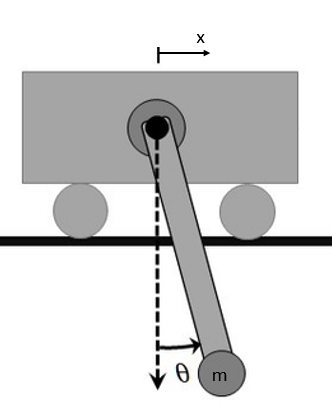
\includegraphics[width=.8\linewidth]{pendulumoncart.png}
		\captionof{figure}{Depiction of the pendulum placed on the cart \cite{Quanser}}
		\label{fig:pendulumoncart}
	\end{minipage}%
	\begin{minipage}{.5\textwidth}
		\centering
		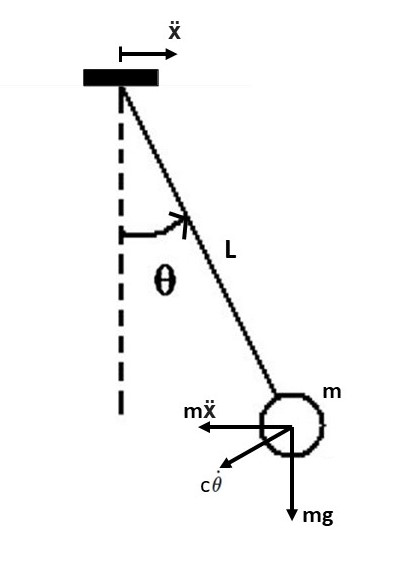
\includegraphics[width=0.8\linewidth]{VLDpendulum.jpg}
		\captionof{figure}{Free body diagram of the pendulum \cite{Researchgate}}
		\label{fig:VLDpendulum}
	\end{minipage}
\end{figure*}


\subsection{State-space equation for the nonlinear model}

\subsection{Linearization of the model}

\subsection{Determination of the pendulum length}

\subsection{Discretization}


\bibliographystyle{plain}
\bibliography{bibliography}

\end{document}